\section{Introduction}
Our intuition was formed in three dimensions and is often misleading in higher dimensions. Consequently, we often resort to unsound dimensional analogy in which our observations from two or three dimensions are empirically assumed to generalise to higher dimensions. In Volume 1 of the yearly release of \textit{What’s Happening in the Mathematical Sciences} two such incorrect conjectures proposed about higher dimensions were presented in the chapter \textit{Disproving the Obvious in Higher Dimensions} \cite{Cipra_1993}. As an example for the reader to explore their own high-dimensional intuition, the end of the chapter featured a box titled \textit{Here's Looking at Euclid}. Within the box, without much elaboration, was the IK-Sphere Problem.

\section{The IK-Sphere Problem}
Suppose a square with side length 2 units in two-dimensional space has unit circles (circles with radius 1 unit) on each of its vertices as in Figure \ref{fig:2d_Setup_IK_Sphere}.
\begin{figure}[h]
    \centering
    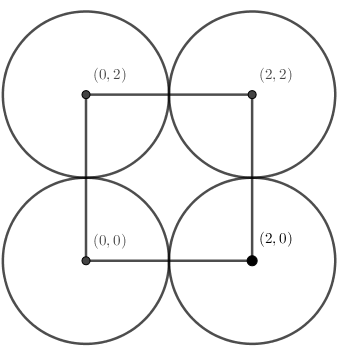
\includegraphics[width=0.4\textwidth]{images/2D.png}
    \caption{\label{fig:2d_Setup_IK_Sphere}Setup for the 2D IK-Sphere problem.}
\end{figure}
\\Now, inscribe a circle with centre matching that of the square that `kisses' the unit circles (see Figure \ref{fig:2d_IK_Sphere}). This inner circle will be named an IK-Sphere (Inscribed Kissing Sphere) for the purposes of this essay.
\begin{figure}[h]
    \centering
    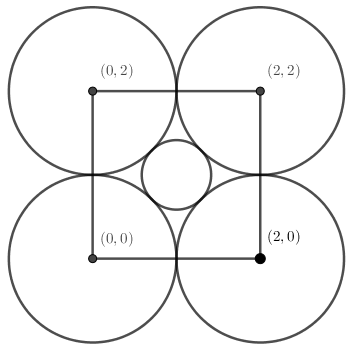
\includegraphics[width=0.4\textwidth]{images/2D IK.png}
    \caption{\label{fig:2d_IK_Sphere}The 2D IK-Sphere problem.}
\end{figure}
\\The definition of a sphere and cube can be generalised across all dimensions so that we may extend the IK-Sphere into higher dimensional space. We will name these the $n$-sphere and $n$-cube respectively.

\begin{definition}[$n$-Sphere]
    An $n$-sphere is a generalised 3D sphere (3-sphere) to $n$-dimensional space, created by all points equidistant (specified by a radius) from a common centre point. For example, a circle is a 2-sphere, a line is a 1-sphere, and a point is a 0-sphere.
\end{definition}

\begin{definition}[$n$-Cube]
    An $n$-cube generalises the cube (3-cube) to $n$ dimensions. It is created by extending an ($n-1$)-cube in a direction perpendicular to itself (see Figure \ref{fig:how to n cube}).
    \begin{figure}[h]
    \centering
    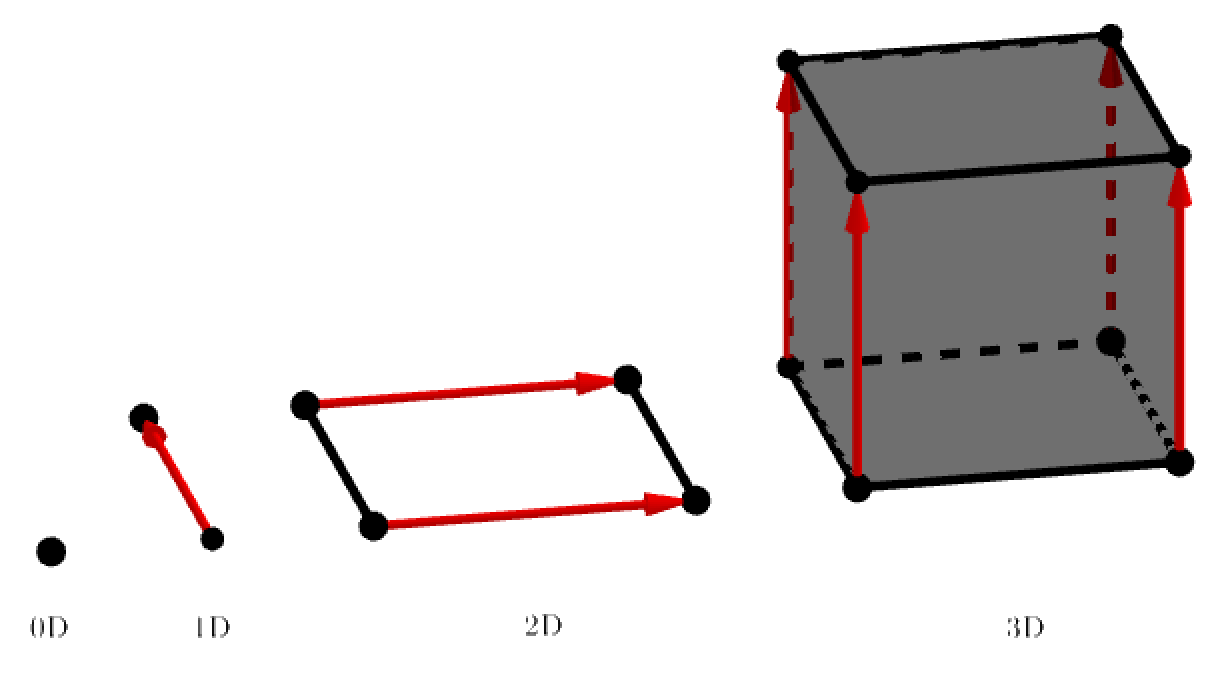
\includegraphics[width=0.8\textwidth]{images/how to make n sphere.png}
    \caption{\label{fig:how to n cube}Extending an ($n-1$)-cube in a perpendicular direction to create an $n$-cube}
    \end{figure}
\end{definition}
Abiding by these definitions, we repeat the process to create an IK-Sphere in three dimensions (see Figure \ref{fig:3d_IK_Sphere}) and find that the radius of the IK-Sphere increases (see Figure \ref{fig:compare IK spheres}). 

\begin{figure}[h]
    \centering
    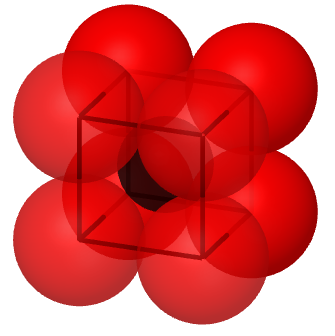
\includegraphics[width=0.5\textwidth]{images/3D IK.png}
    \caption{\label{fig:3d_IK_Sphere}3D IK-Sphere.}
\end{figure}

\begin{figure}[h]
    \centering
    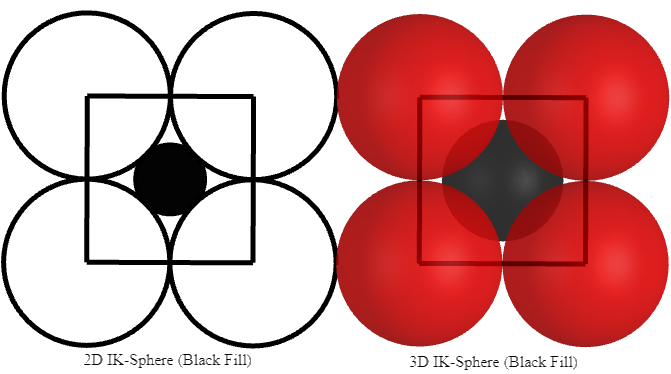
\includegraphics[width=0.8\textwidth]{images/compare ik spheres.png}
    \caption{\label{fig:compare IK spheres}Comparing radius of 2D IK-Sphere to 3D IK-Sphere.}
\end{figure}

Without explanation as to why, the \textit{Here's Looking at Euclid} box states that as the number of dimensions increase, the radius of the IK-Sphere increases without bound -- contrary to one's assumption that the radius will approach touching the bounding cube but never exceed it. Thus, this prompted the research question:
\researchquestion{}














